\scanpage{401}\mspage{140}
un isom fonctoriel en $X$ (passage au chemin
opposé)
\[
\begin{tikzpicture}[baseline=(f.base)]
\node[inner sep=3pt] (f) {$\mathrm{Ch}_{\infty}^{\underline t}(X)\xrightarrow{c\unsure{\mathrel{\vdash\!\dashv}|\mapsto}c^{\circ}}\underline{\mathrm{Ch}}_{\infty}^{\underline t^{\circ}}(X)$};
\draw (f.north west)--(f.south west)--(f.south east)--(f.north east);
\end{tikzpicture}
\]
% slanted
\margin{cf page 143 pour le passage de $\underline t$ à $\underline t^{-}$}
qui ``échange source et but''. Bien sûr, on
a intérêt à prendre $\unsure{\underline{\bar t}|\underline t}$ tel qu'on ait
$\underline t=\underline t^{\circ}$ (c'est ce que j'avais fait, par un
\unsure{sûr|sain} instinct, dès le début de $\overline{\underline{\mathrm V}}$), de
sorte qu'on a \unsure{un|une} \inserted{foncteur} involutif canonique
\[
\underline{\mathrm{Ch}}_{\infty}(X)\xrightarrow{c\mathrel{\vdash\!\dashv}c^{\circ}}\underline{\mathrm{Ch}}_{\infty}(X)
\]
(je laisse tomber à nouveau l'exposant $\underline t$),
qui ``échange source et but''. Donc on trouve,
à isom. \inserted{can.} près, la ``$=$'' factorisation de $f\colon X'\unsure{\relbar|\to}X$
en $\bar f\circ\alpha$, \deleted{\unsure{que}} si on fait comme \unsure{dessus} page
38, pour définir $\overline{X'}$ et $\alpha$, ou si dans ce
diagramme on intervertit les rôles de $\sigma$ et
de $\beta$.

Enfin

$4^\circ$) Si
\[
c\colon \unsure{a|\bullet}\longrightarrow b
\]
est un chemin quelconque dans $X$, on
% slanted
\margin{\unsure{Surtout} pour se borner au cas où $c$ serait un des $t_n$ !}
voudrait en conclure une \unsure{iso.} dans
$\mathrm{Hot}$ (de ``transport par $c$'')
\[
\overline{X'}_a\xrightarrow{\substack{\bar c\\[-2pt]\sim}}\overline{X'}_b,
\]
% slanted
\margin{décrire quand même l'effet sur les $\pi_0$ !}
avec bien sûr transitivité pour la composition,
% archive sheet number: 400
